\section{Description}

% Summarize pair-HMMs. Brief, comment typically used but move onto FST right away
Statistical alignment is typically performed using pairwise hidden Markov models
(pair-HMMs).
Pair-HMMs are computational machines that have the ability to rigorously model
molecular sequence evolution and can calculate the probability that two
sequences are related, represented $P(X, Y)$ \parencite{yoon_2009_hmm}.
However, a limitation of pair-HMMs is the ability to only model the evolution
of two related sequences from an unknown ancestor.

Finite-state transducers (FSTs) have the same benefits as pair-HMMS with the
additional ability to generate a descendant sequence given an ancestral one.
Properly weighted, an FST can calculate the probability that a sequence $Y$
(descendant) evolved from sequence $X$ (ancestor), represented $P(Y | X)$.
Furthermore, the existence of well-established algorithms for combining FSTs in
different ways \parencite{bradley2007transducers} allows the design of complex
models by combining simpler FSTs.
A powerful and versatile algorithm for comparative sequence analysis is
composition, which consists of sending the output of one FST into the input of a
second FST.
The FST model implemented in COATi is designed by composing smaller FSTs, each
representing a specific process.

Pairwise alignment in COATi is implemented via the Evolution FST (Fig.
\ref{fig:evolution-fst}), based on existing transducers (e.g.
\cite{holmes2001evolutionary}).
The Evolution FST is formed by composing a substitution FST that encodes a 64x64
codon model (Fig. \ref{fig:evolution-fst}-a) and an indel FST that models
insertions and deletions, including frameshifts (Fig. \ref{fig:evolution-fst}-b).
The substitution models available are Muse and Gaut \parencite{muse_gaut_1994}
(MG94) and the Empirical Codon Model \parencite{kosiol_ECM_2007} (ECM).
The innovation of the Evolution FST with respect to other transducers is the
combination of a codon substitution model that allows stop codons with gaps that
can occur at any position of any length.

\begin{figure}[h!]
\begin{framed}
\centering
    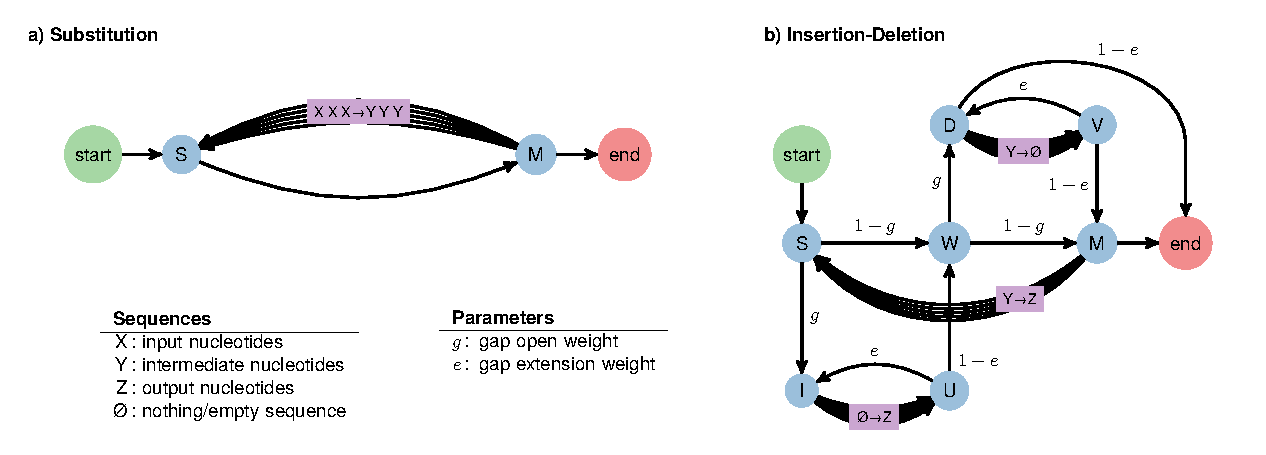
\includegraphics[width=\textwidth]{fig-evolution-fst.pdf}
    \caption{The Evolution FST is assembled by composing a substitution FST and
    an indel FST. Each node represents a state in an FST while arcs display
    possible transitions between states (and their weights). (a) The
    substitution FST encodes a 64x64 codon substitution model with 64 arcs from
    M to S. (b) The indel FST allows for insertions (I to U) and deletions
    (D to V). Contiguous insertions and deletions are always arranged for
    insertions to precede deletions to limit equivalent alignments.}
    \label{fig:evolution-fst}
\end{framed}
\end{figure}


% FST implementation
% A path through the FST that \green{results} from composing both sequences with
% the Evolution FST represent a pairwise alignment.
% To find the most \green{probable/likely} alignment we must find the shortest
% path through.
The alignment FST is the result from composing both sequences with the Evolution
FST.
Any path through the alignment FST represents a pairwise alignment, while the
shortest path corresponds to the best alignment.
All FST operations including model development, composition, search for the
shortest path, and other optimization algorithms are performed using the C++
openFST library \parencite{allauzen2007openfst}.

% However, composing large FSTs is an expensive operation and can be prohibitive.
% Despite the existence of efficient C++ FST libraries (e.g. openFST
% \cite{allauzen2007openfst}), runtime is still limiting for sequence pairs longer
% than a few thousand nucleotides each.
% To solve this issue, the search for an optimal path (alignment) is
% reformulated as a dynamic programming problem.

COATi also features a marginal substitution model with substitution probability
matrix

\[P'_{ijp} = \mathlarger{\mathlarger{\sum}}_{cod} \thickspace \begin{cases}
P(i \thinspace | \thinspace cod) \enspace \text{if} \enspace cod_p = j\\
0 \enspace \text{otherwise}
\end{cases} \]

Where $P'_{ijp}$ represents the probability that codon $i$ from the ancestor
sequence changes to nucleotide $j$ of the descendant sequence at position $p$
$\in \{0, 1, 2\}$ of the reading frame.
$P$ is the substitution probability matrix MG94 or ECM.
This model emphasizes the position where the substitution in a codon occurs and
helps restrict the effects of low quality data in the descendant sequence.
In combination with the indel FST alignment with the marginal model can be
implemented using dynamic programming, which results in a significant speed up
with similar accuracy.

% Evolution FST + Q matrix
% Marginal model? - Probably not
% DP - probably not
% 1 figure: FST model? - results table?
